\subsection{Приложение 1. Демонстрация установки}\label{sec:application1}
\begin{figure}[H]
    \centering
    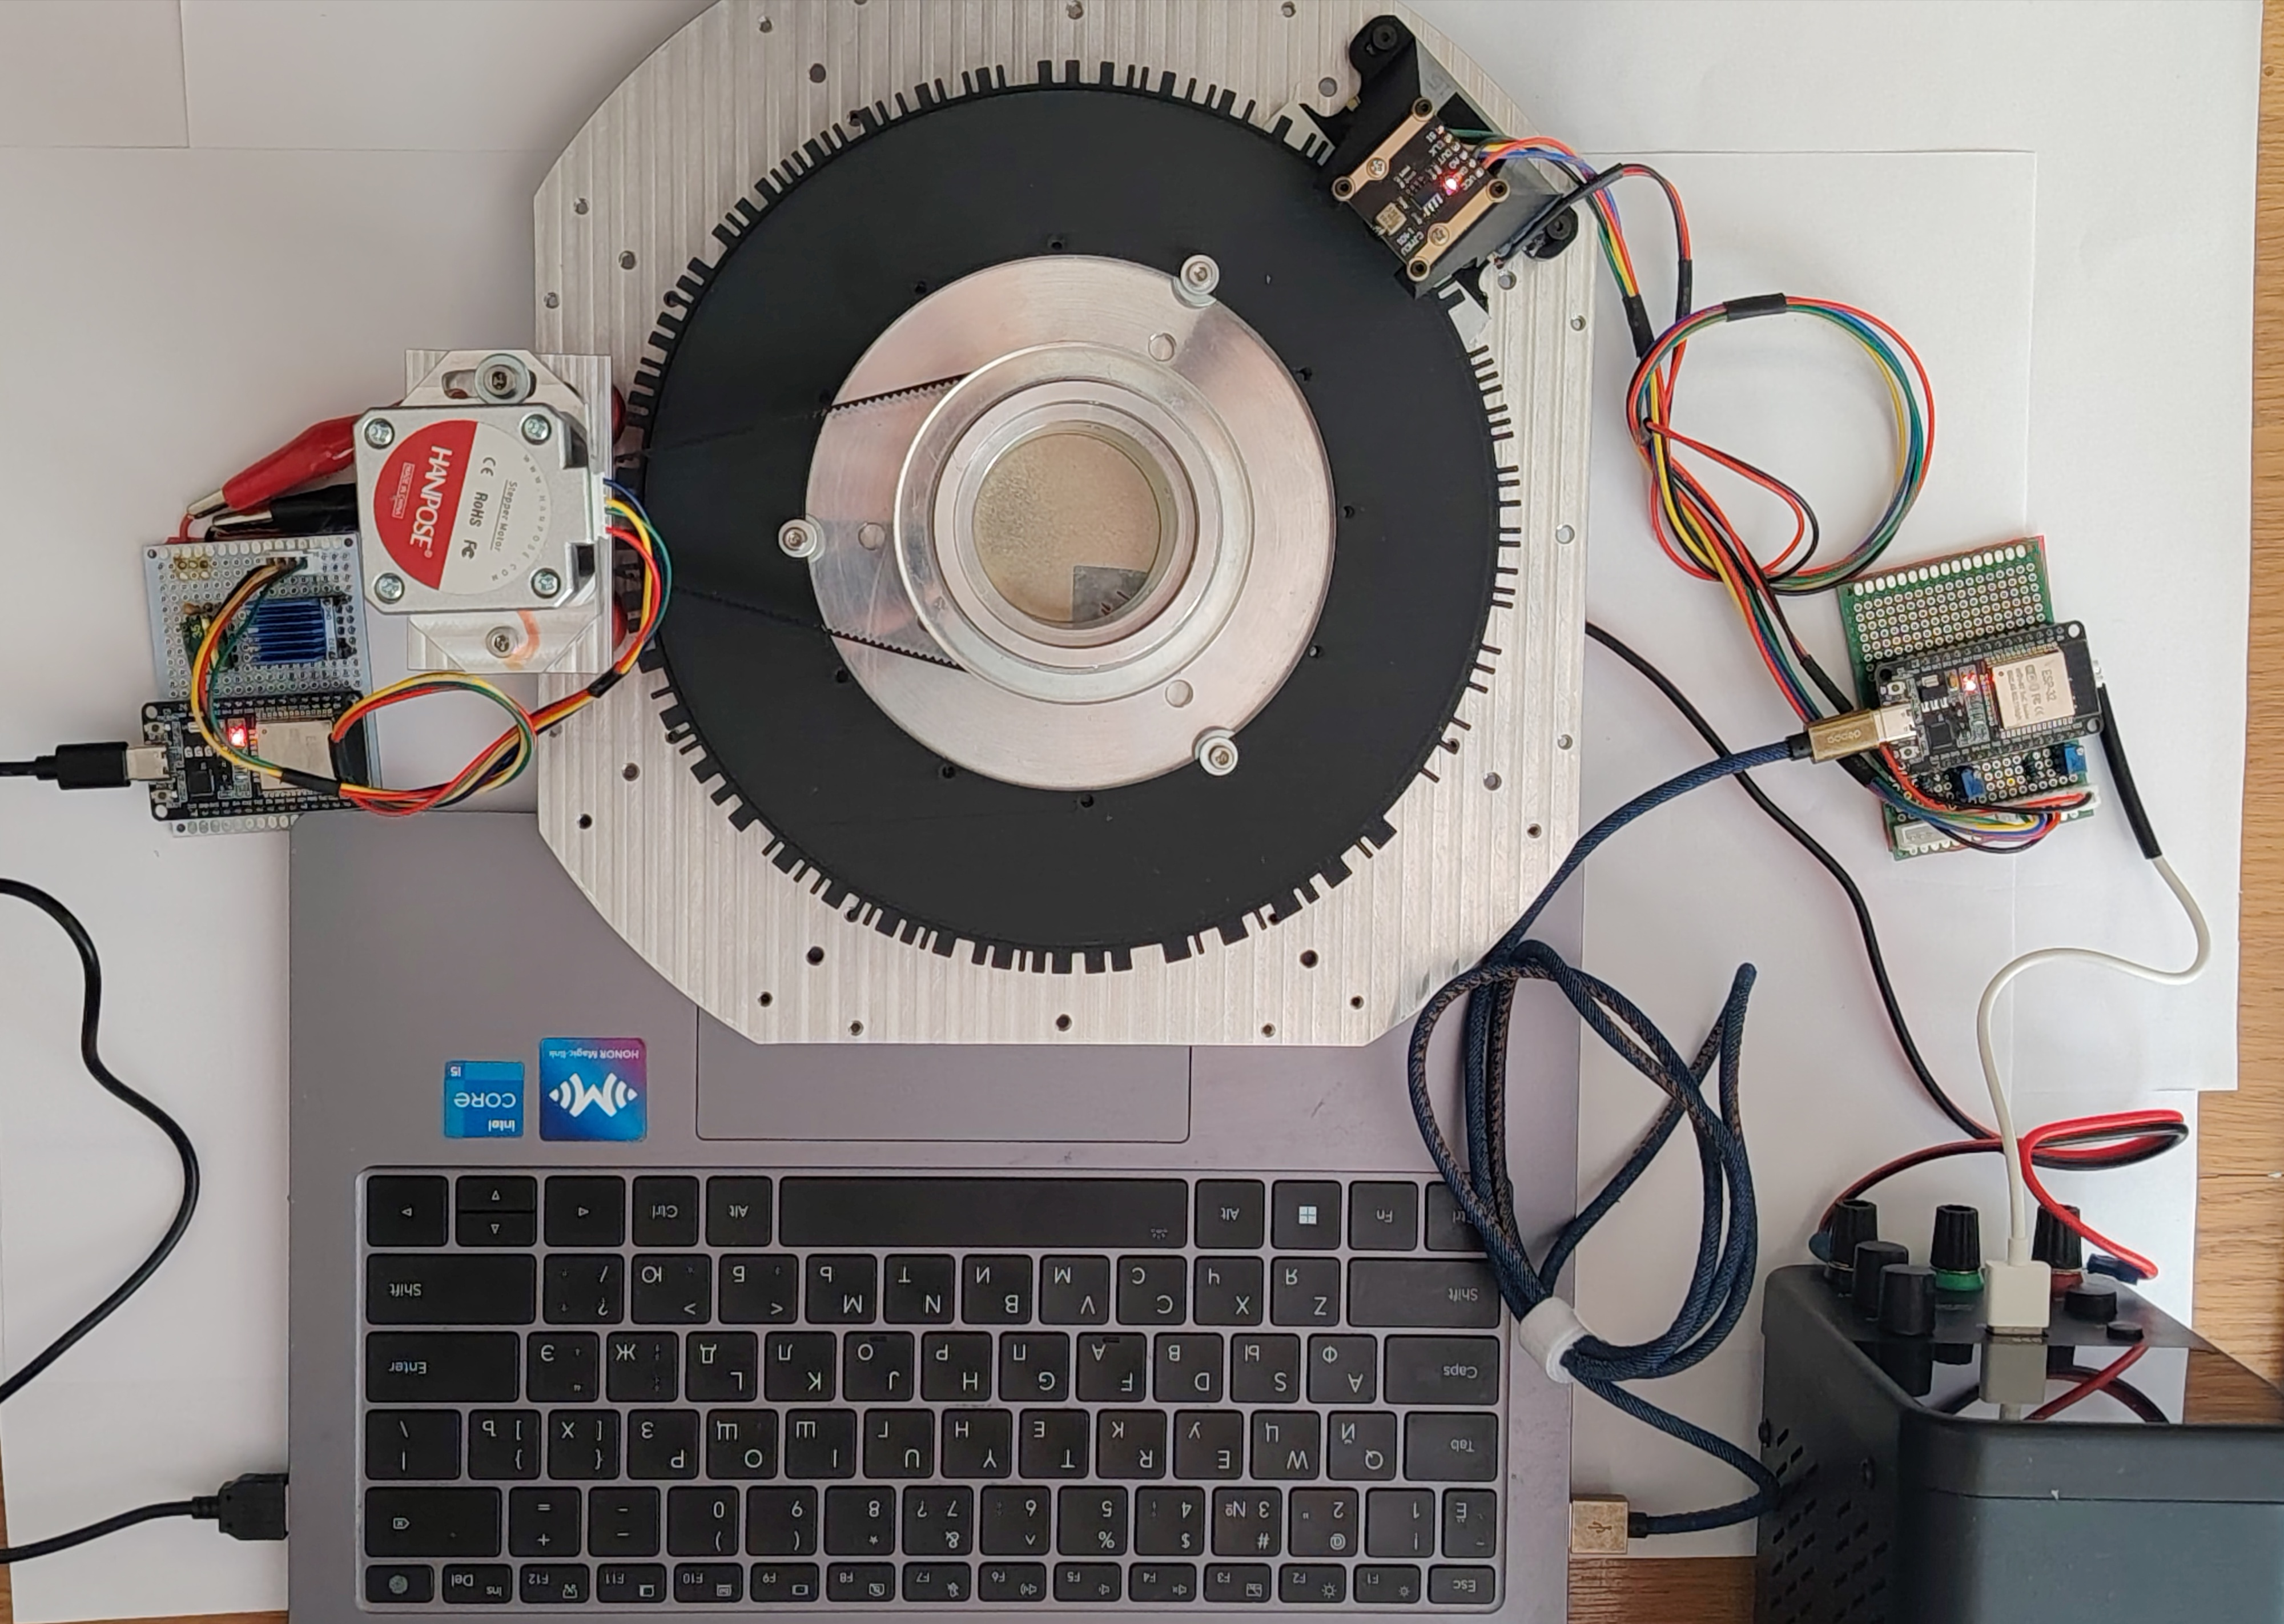
\includegraphics[width=1.2\linewidth, angle=90]{images/установка матовый.jpg}
    \caption{Фото установки (одна головка и компьютер)}
\end{figure}
\begin{figure}[H]
    \centering
    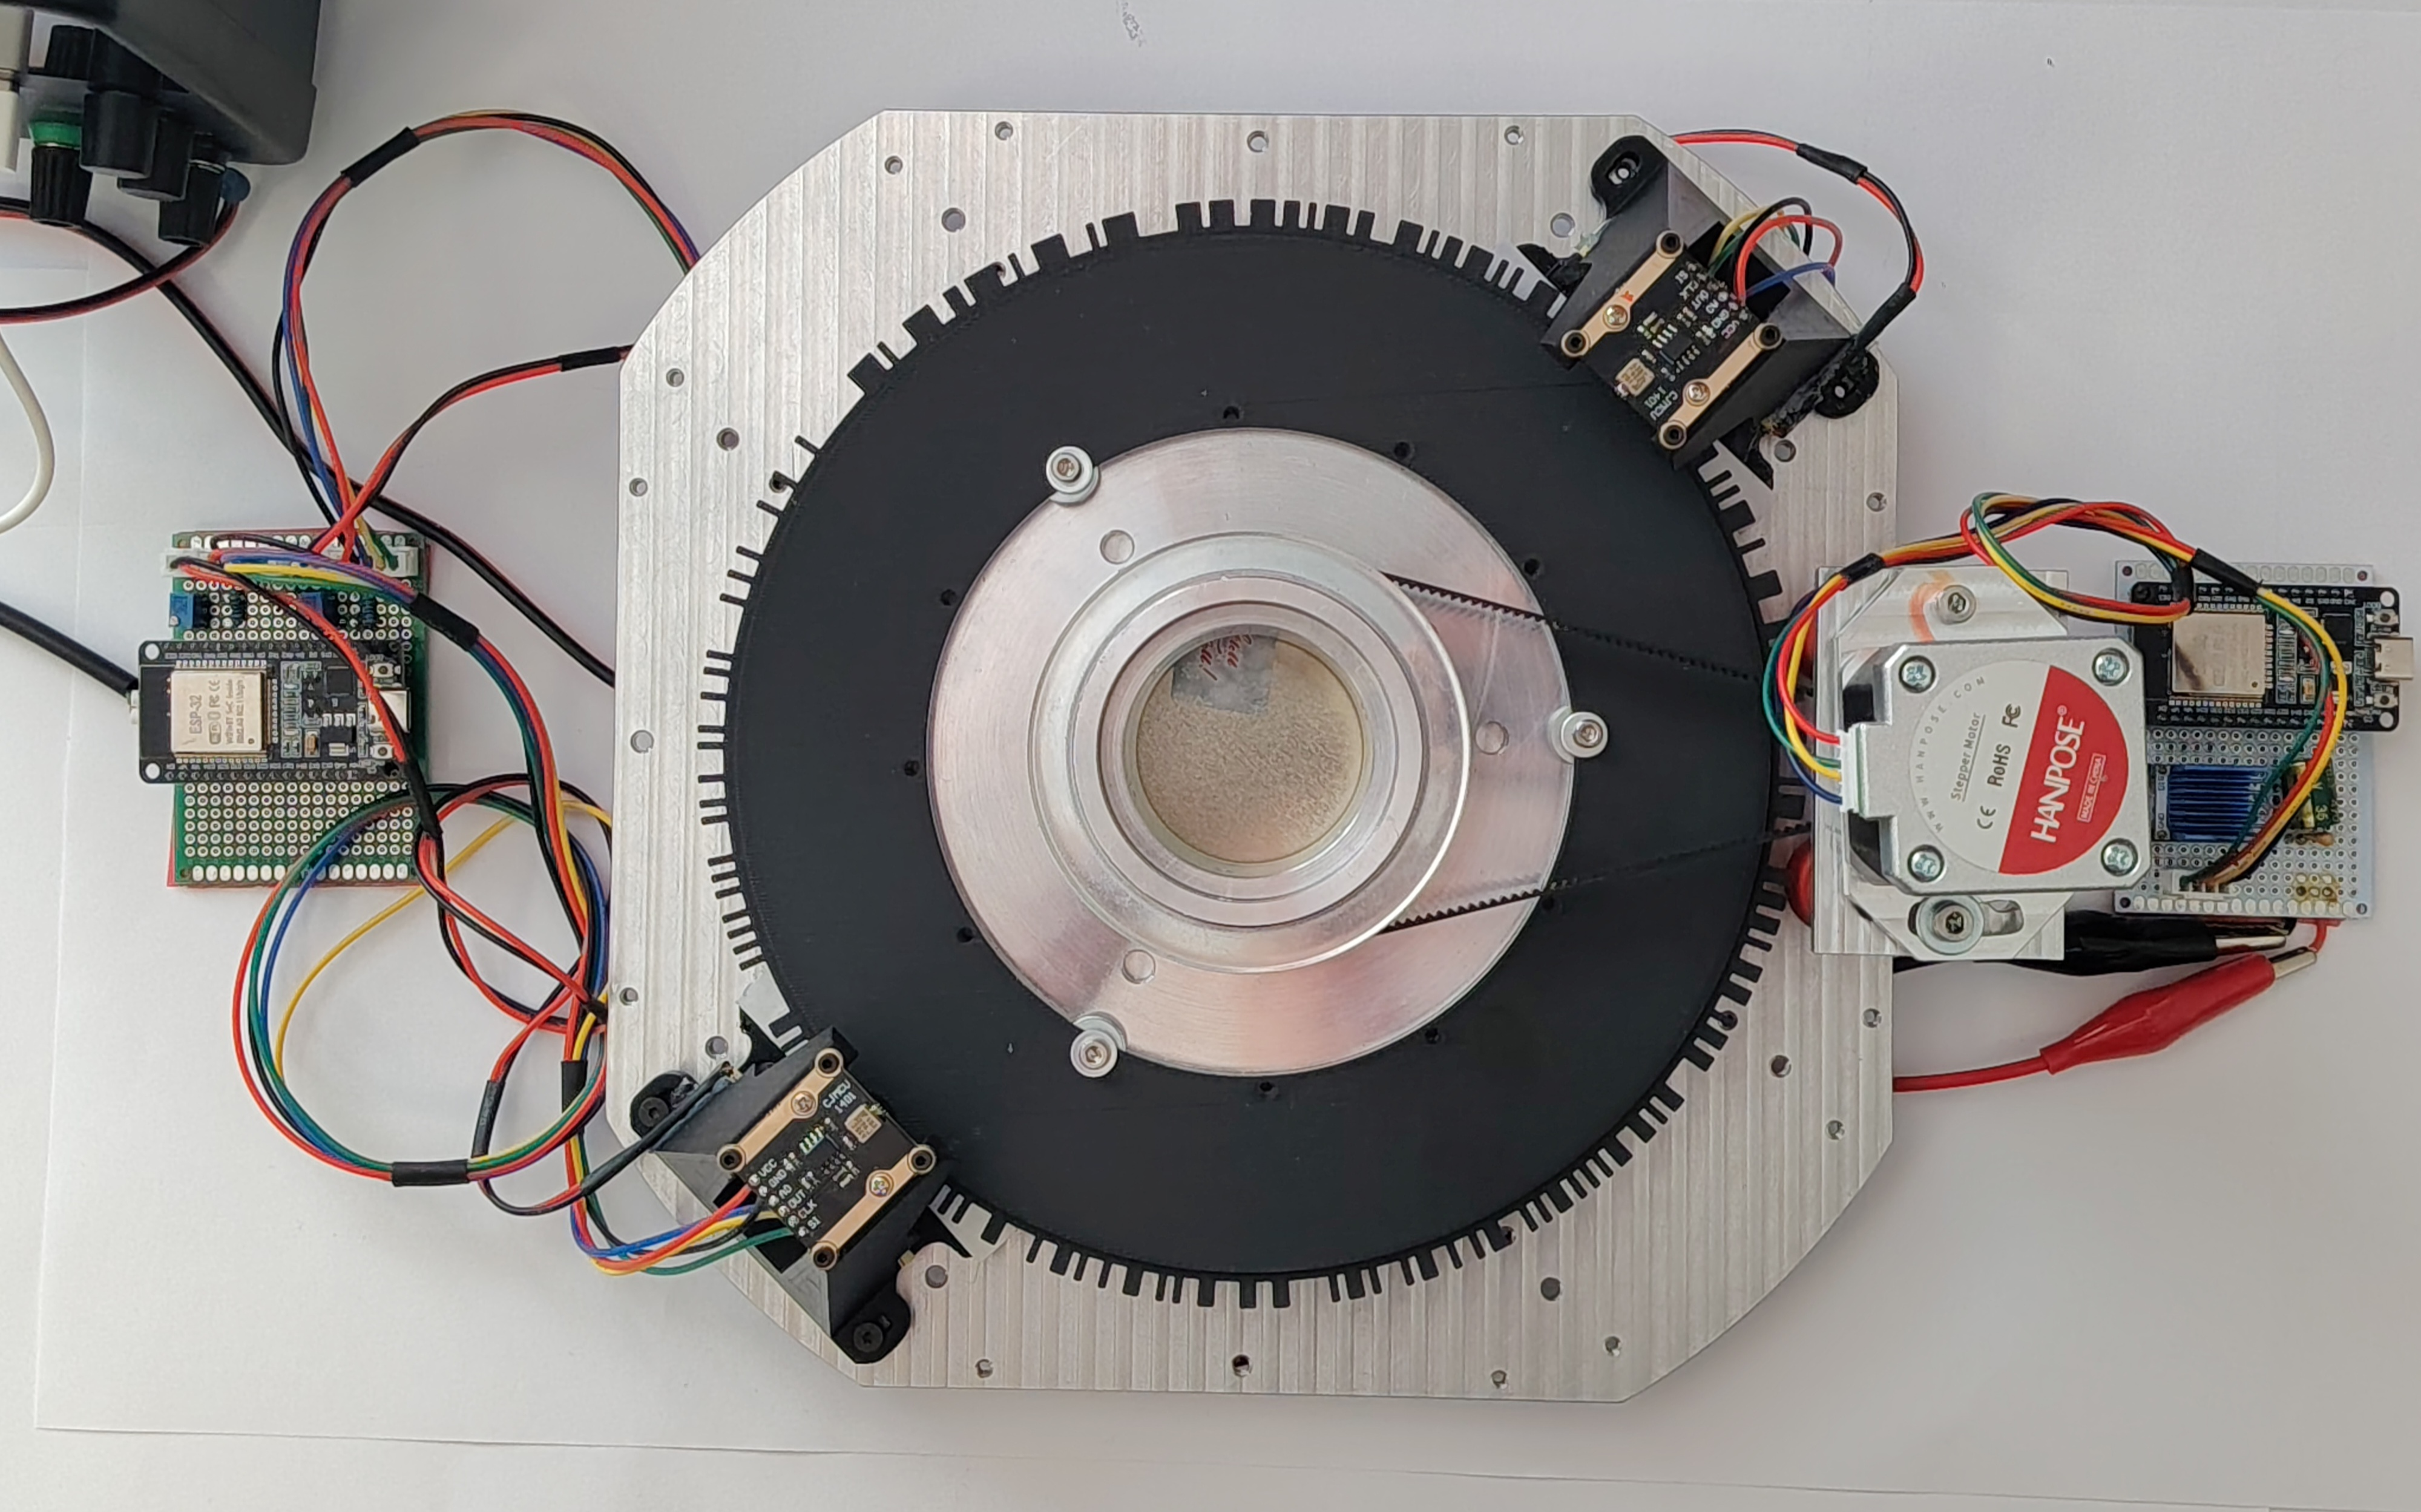
\includegraphics[width=0.9\linewidth]{images/установка две головки.jpg}
    \caption{Фото установки (две головки)}
\end{figure}
\begin{figure}[H]
    \centering
    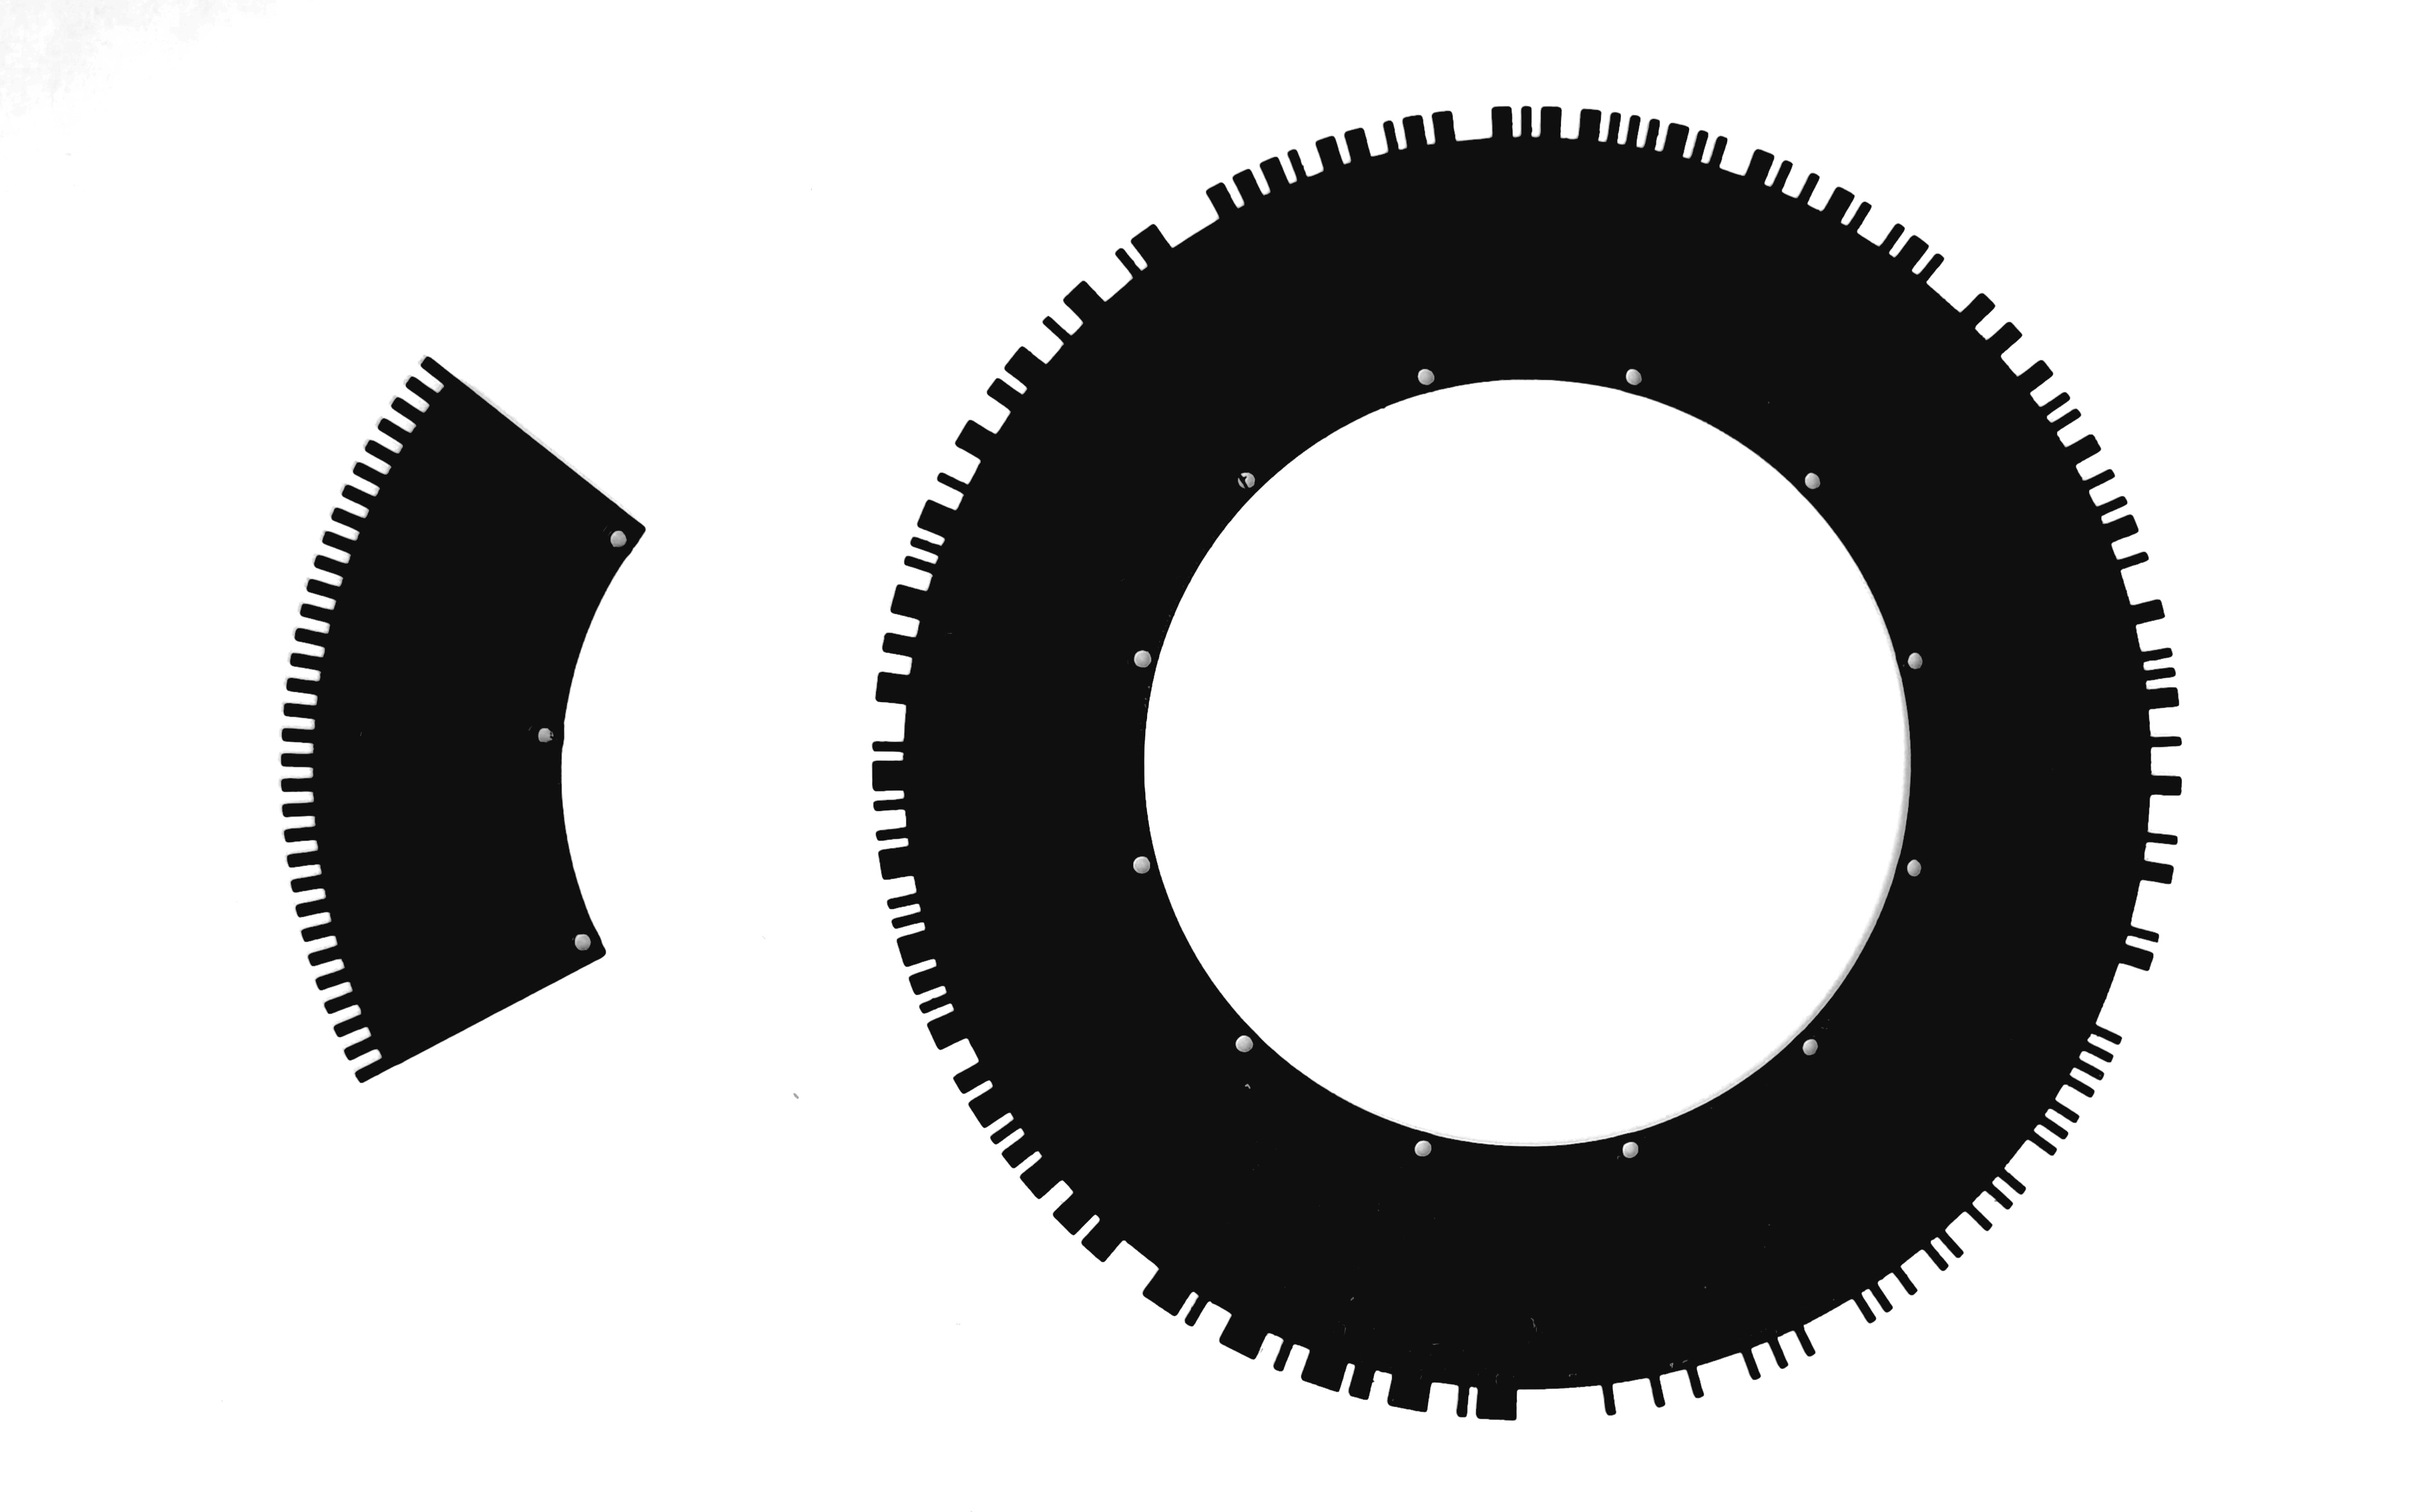
\includegraphics[width=\linewidth]{images/зебра и диск.jpg}
    \caption{Калибровочная <<зебра>> и кодовый диск}
\end{figure}

\subsection{Приложение 2. Демонстрация 3D-модели установки}\label{sec:application2}
\begin{figure}[H]
    \centering
    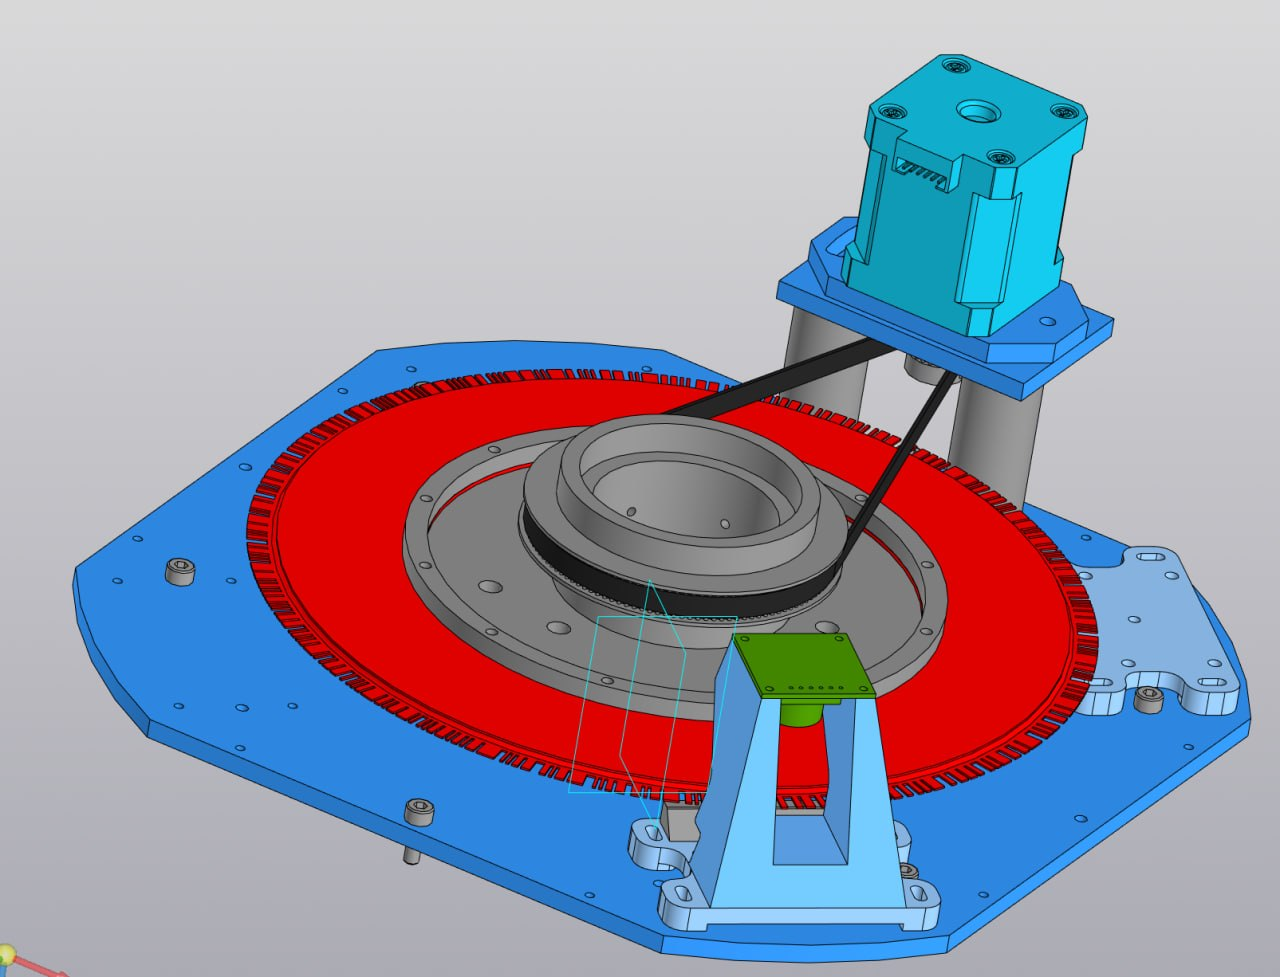
\includegraphics[width=0.9\linewidth]{images/3D модель.png}
    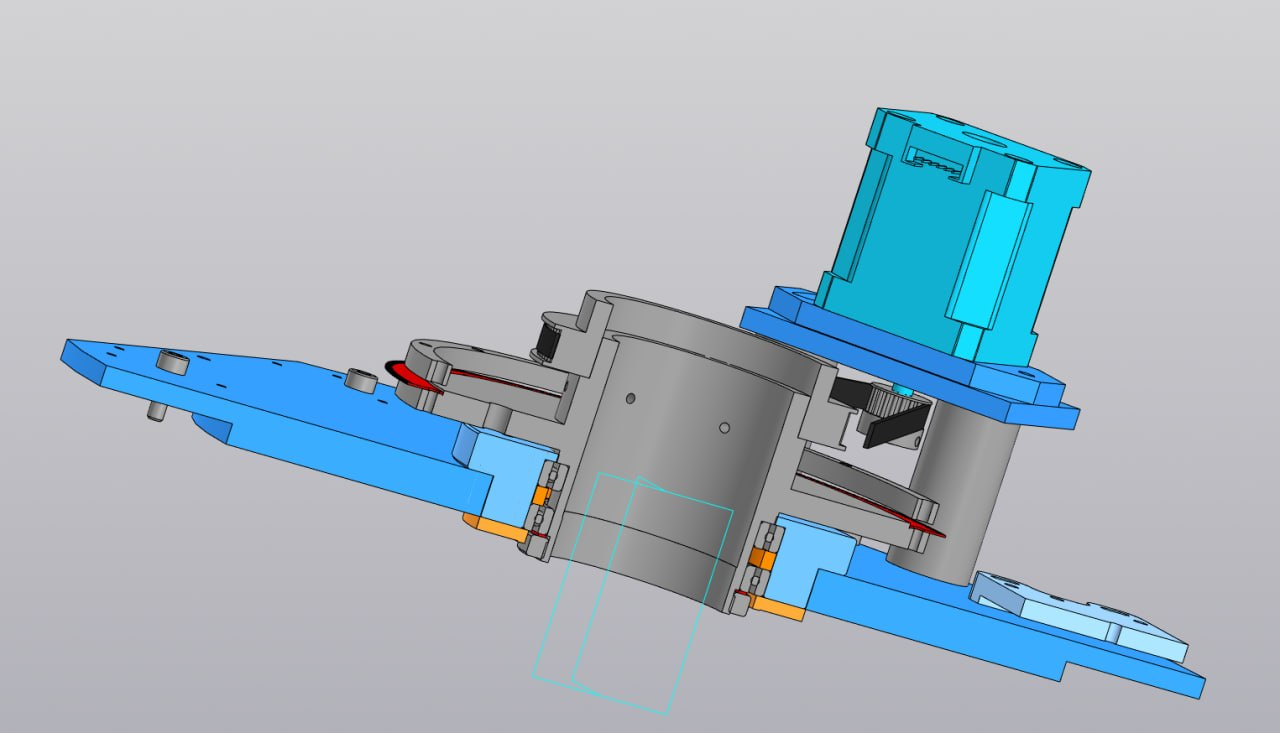
\includegraphics[width=0.9\linewidth]{images/разрез 3D модель.png}
    \caption{3D модель узла энкодера}
\end{figure}

\subsection{Приложение 3. Программный код}
\href{https://github.com/shroomjak/EncoderDecoder.git}{Ссылка на репозиторий}

\subsection{Приложение 4. Диагностические графики точности}\label{sec:application4}
\begin{figure}[H]
\centering
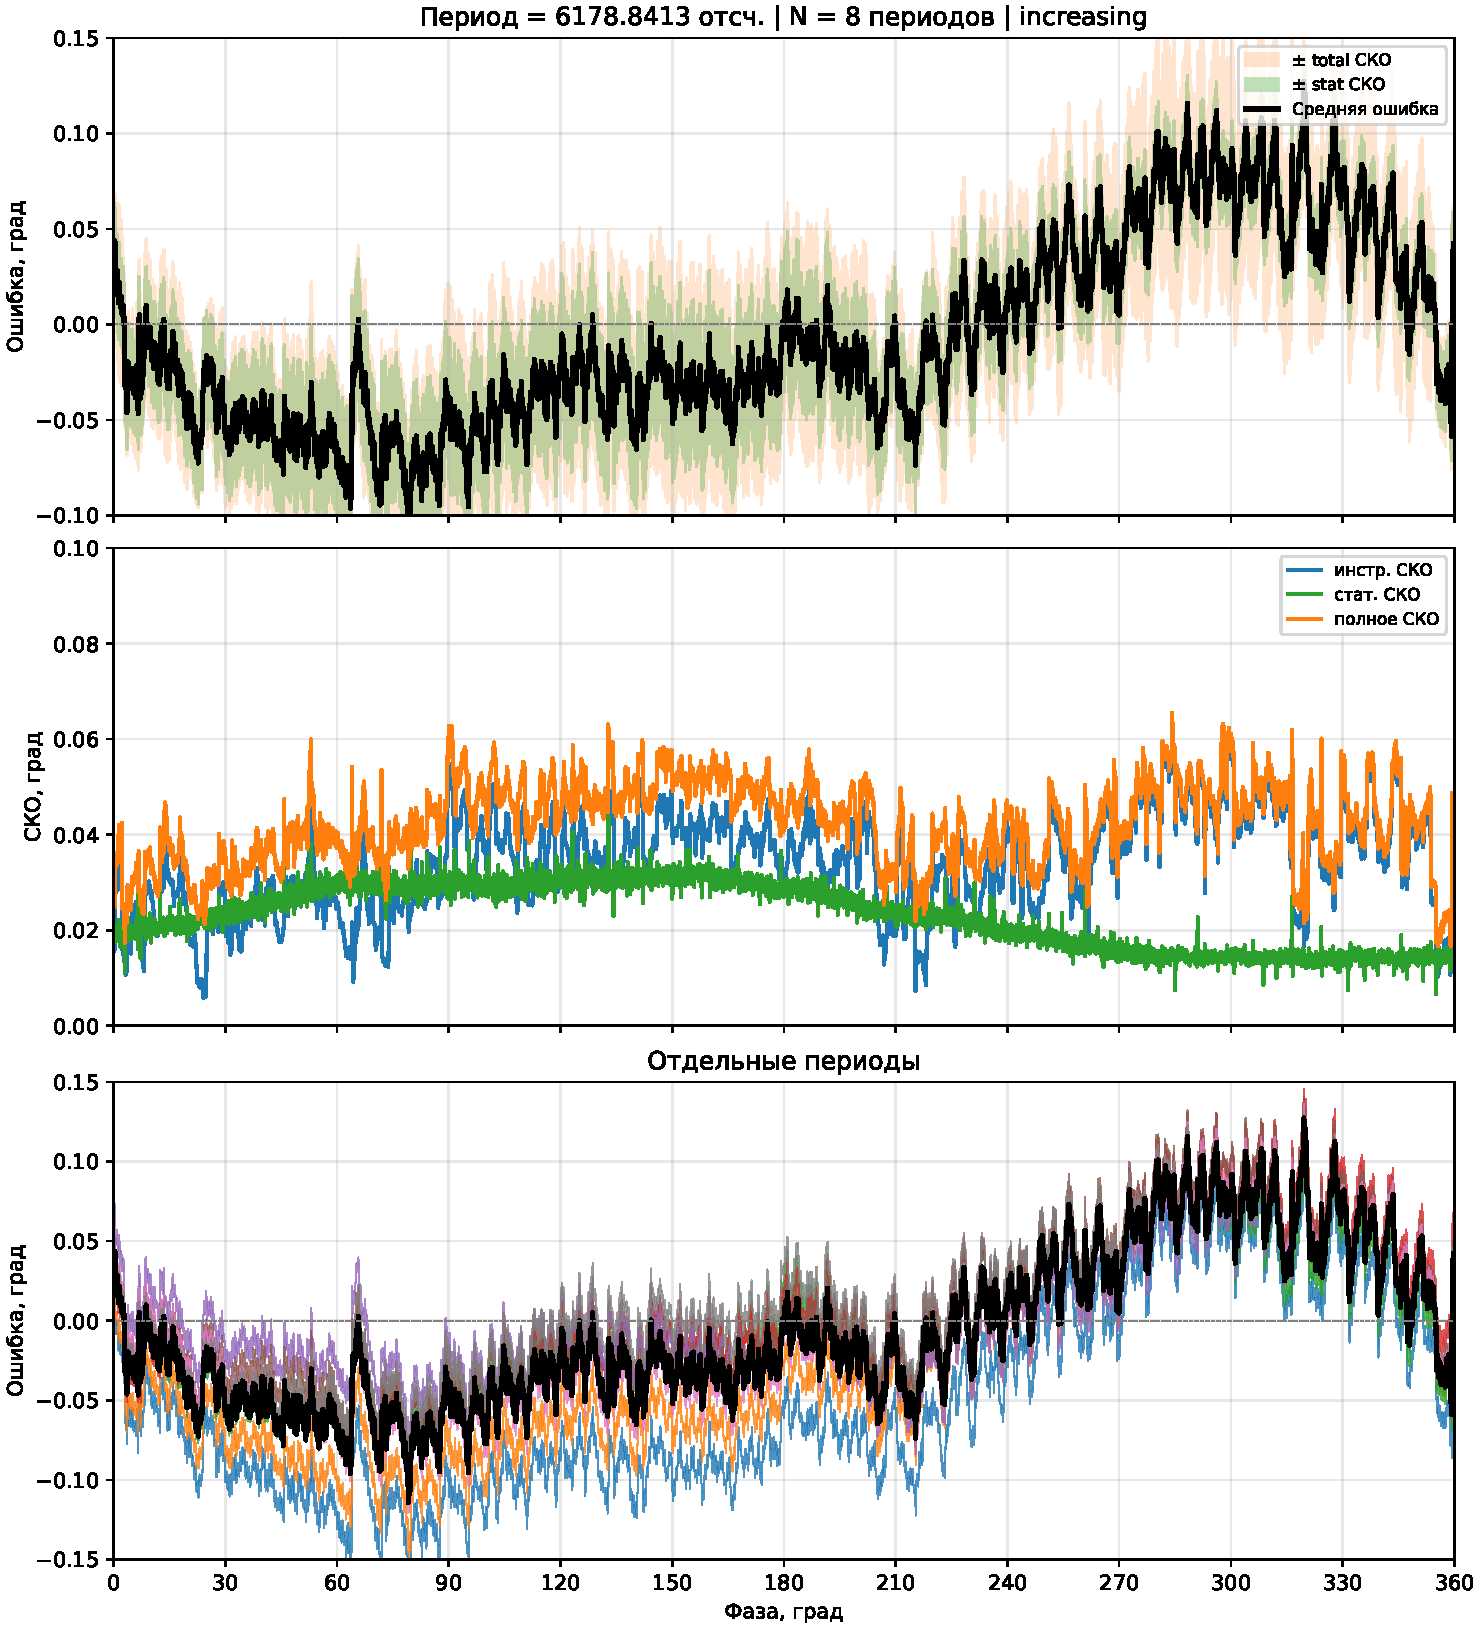
\includegraphics[width=\linewidth]{images/no_trash_2500.pdf}
\caption{Усредненная периодическая ошибка энкодера при скорости 2500 микрошагов в сек. (один оборот за $\sim31$ сек.)}
\label{fig:profile2500}
\end{figure}

\begin{figure}[H]
\centering
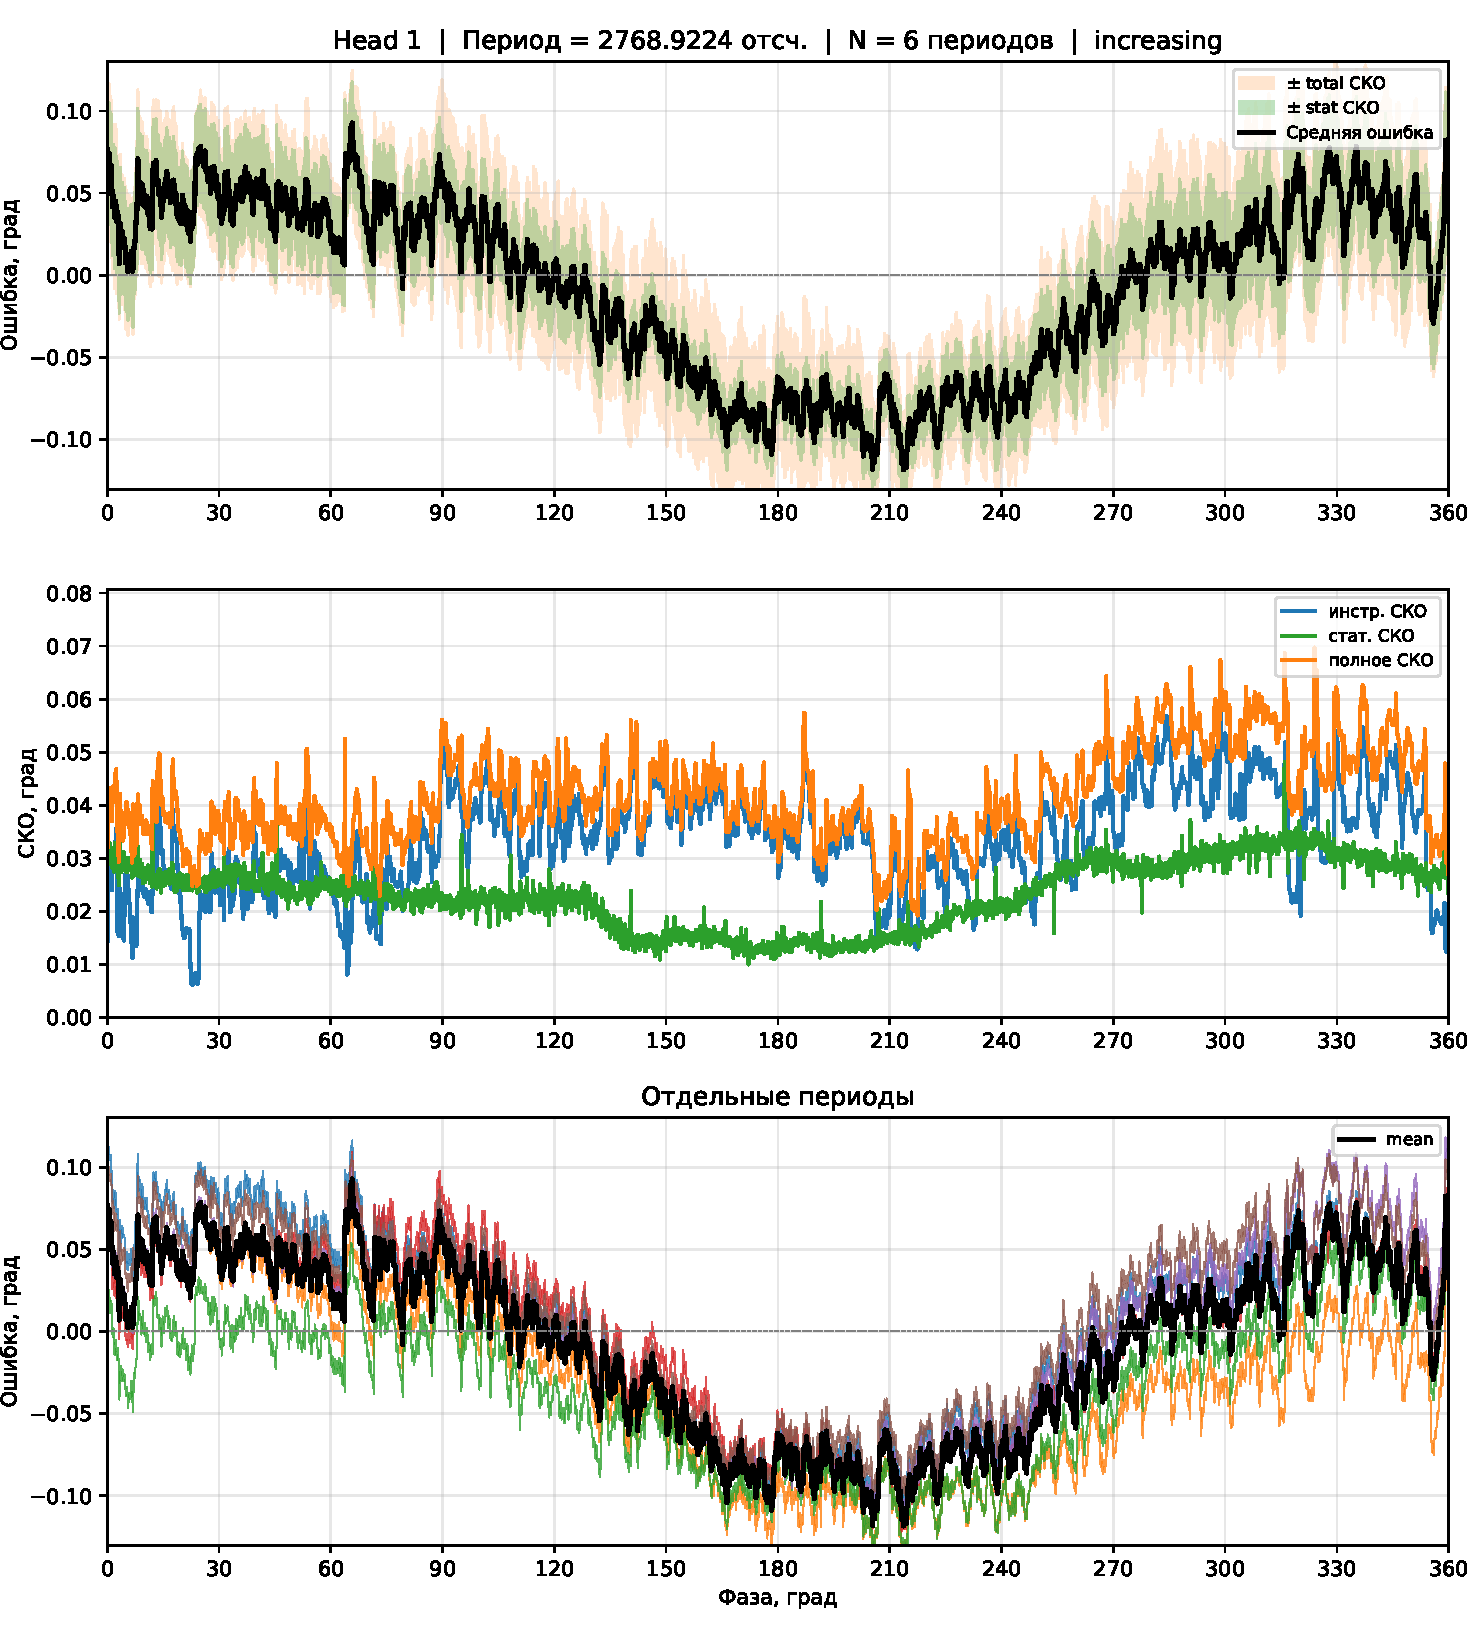
\includegraphics[width=\linewidth]{images/final_10_5000_head1.pdf}
\caption{При скорости 5000 микрошагов в сек. (один оборот за $\sim62$ сек.) с первой головки при вращении согласованно считыванию}
\label{fig:profile5000}
\end{figure}

\begin{figure}[H]
\centering
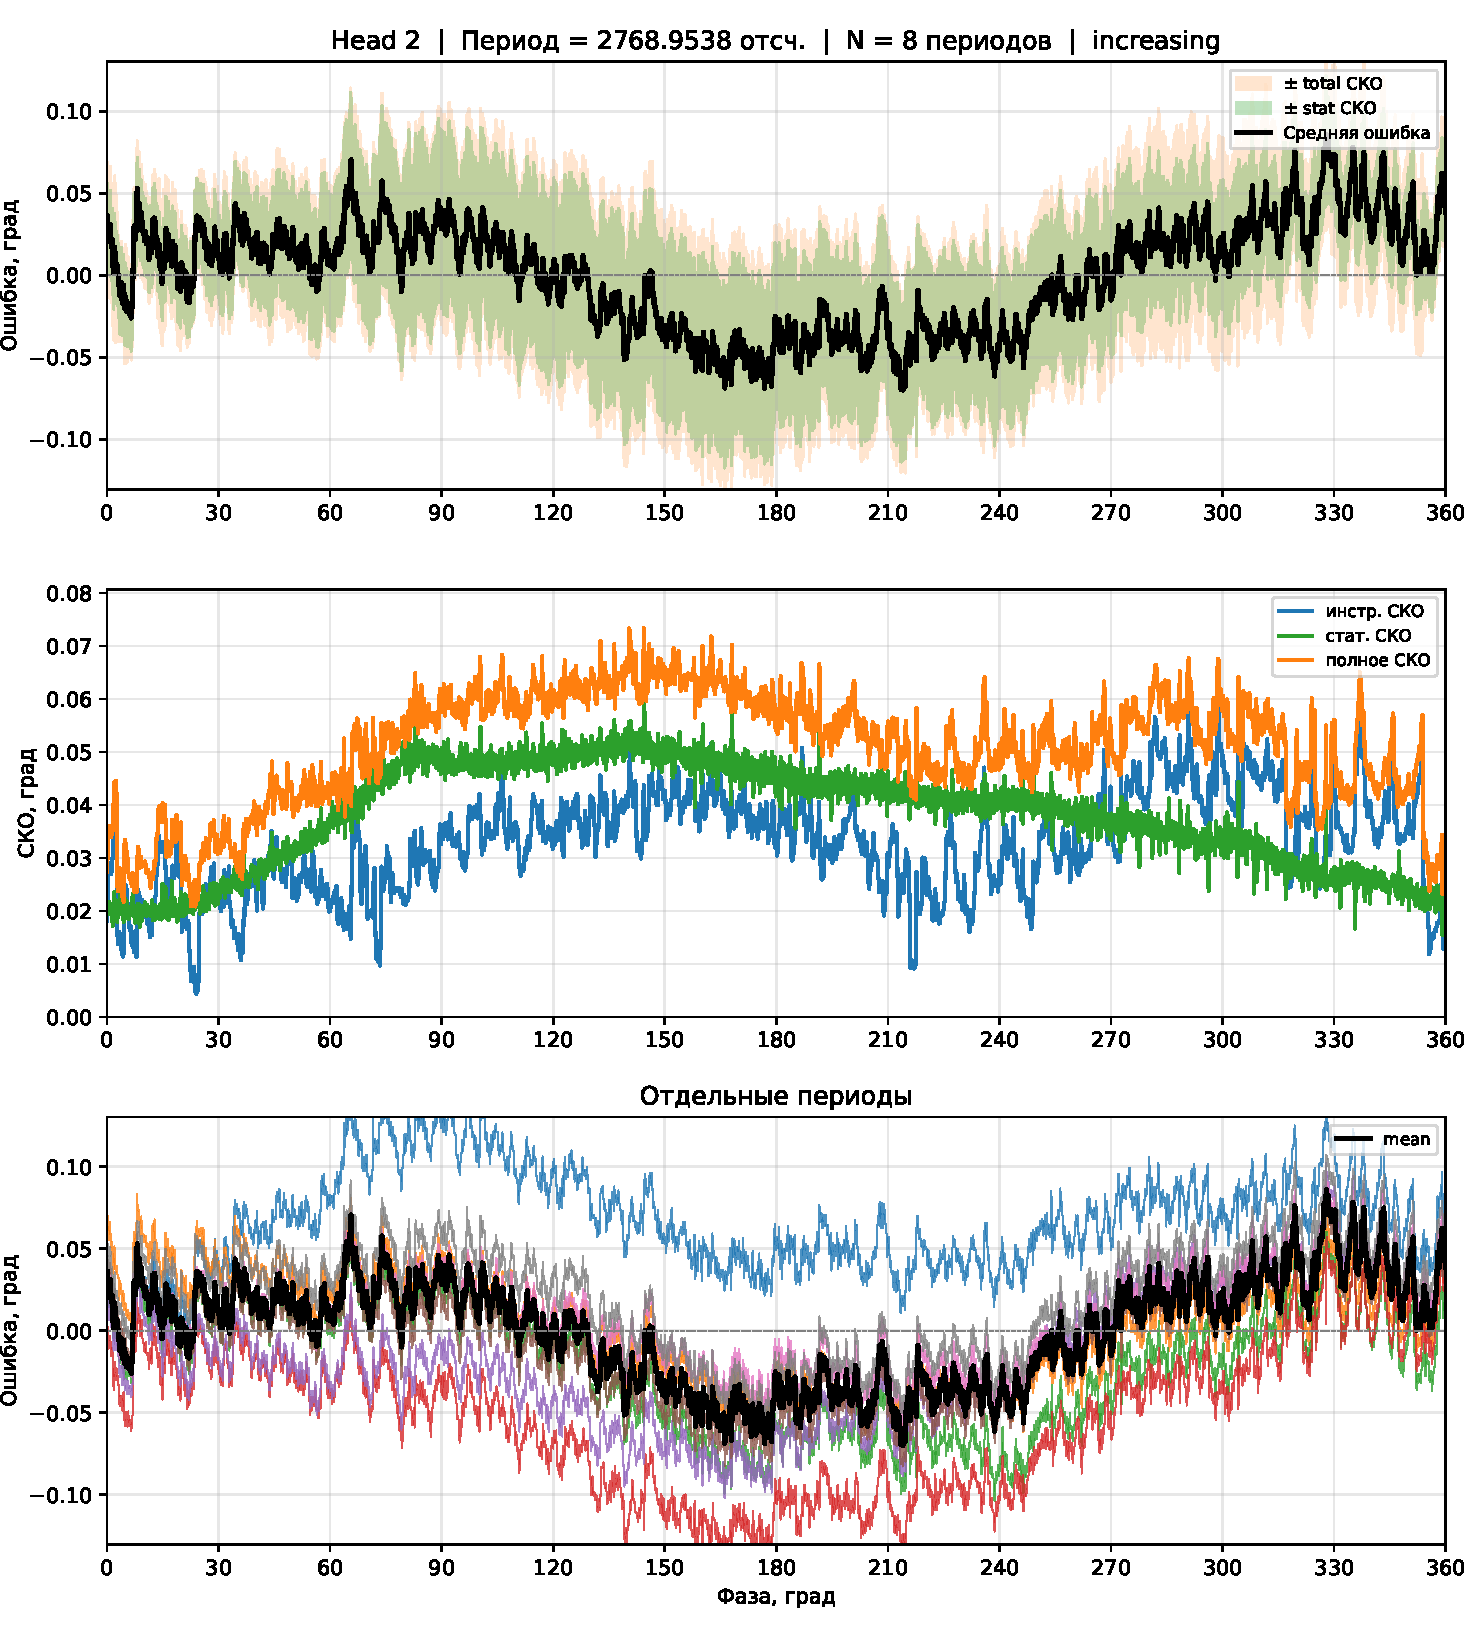
\includegraphics[width=\linewidth]{images/final_10_5000_head2.pdf}
\caption{При скорости 5000 микрошагов в сек. (один оборот за $\sim62$ сек.) со второй головки при вращении согласованно считыванию}
\label{fig:profile5000}
\end{figure}

\begin{figure}[H]
\centering
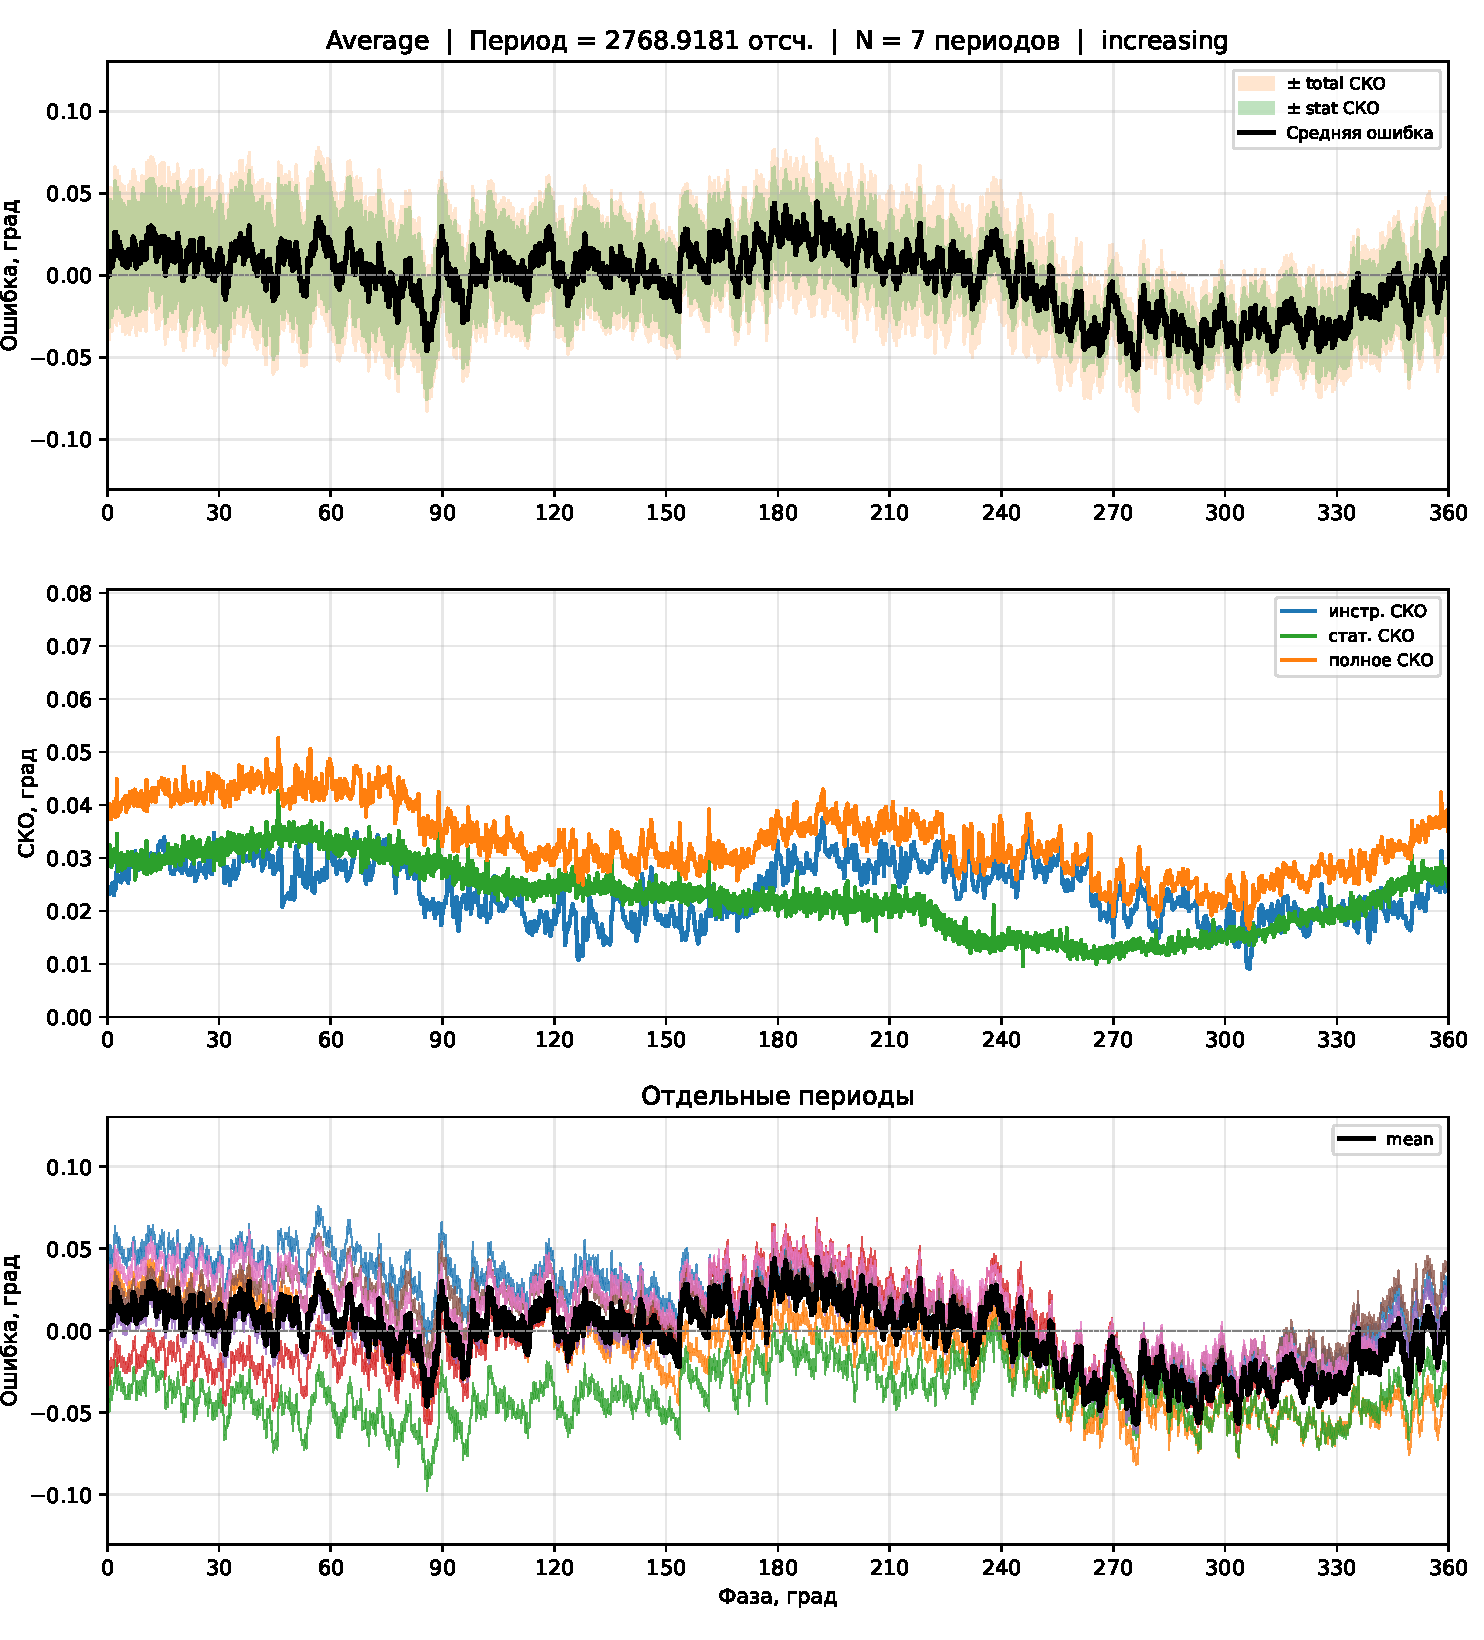
\includegraphics[width=\linewidth]{images/final_10_5000_avg.pdf}
\caption{При скорости 5000 микрошагов в сек. (один оборот за $\sim62$ сек.) круговое среднее показаний двух головок при вращении согласованно считыванию} 
\label{fig:profilerev10000}
\end{figure}

\begin{figure}[H]
\centering
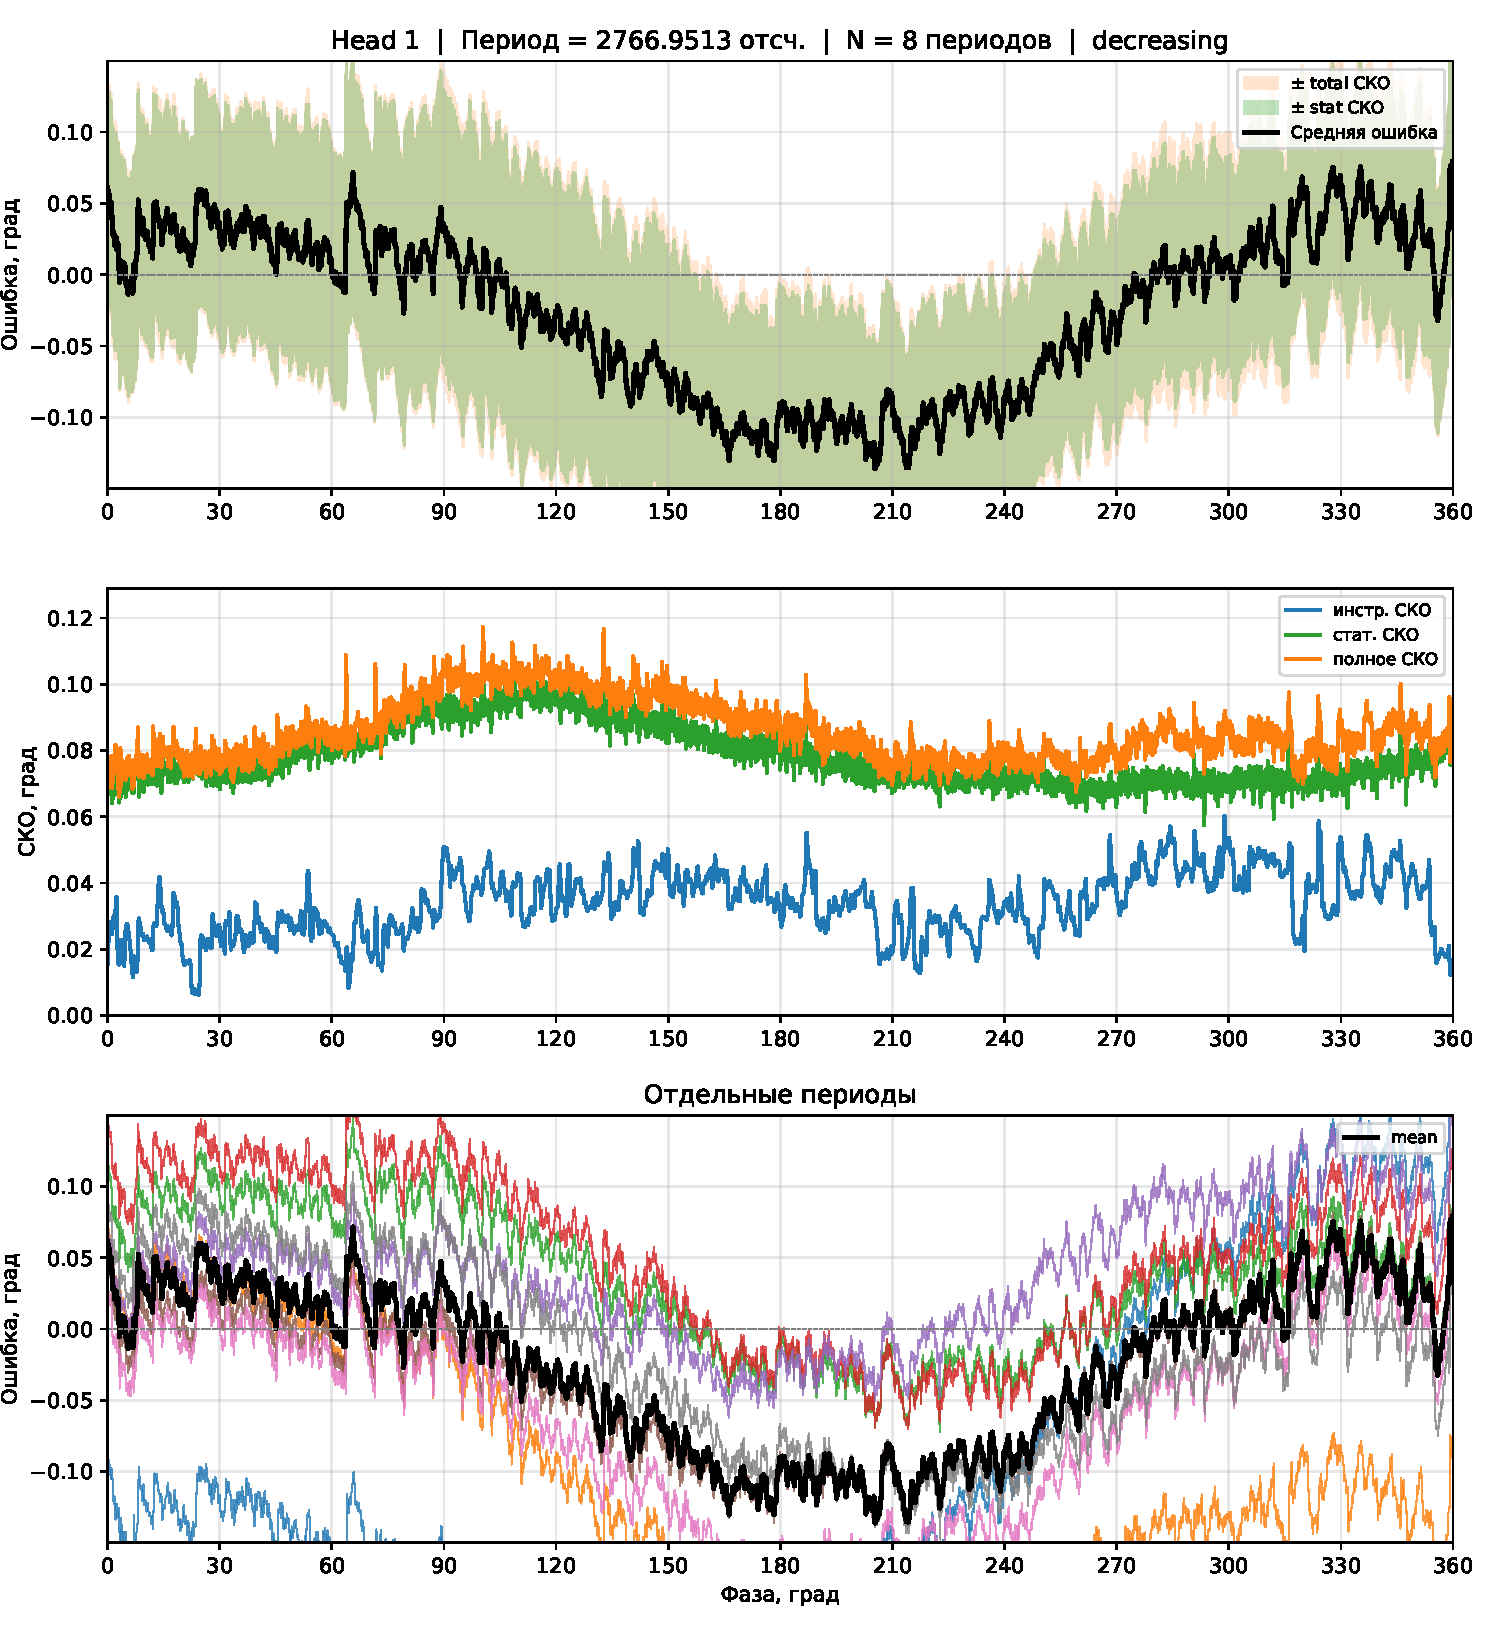
\includegraphics[width=\linewidth]{images/final_reverse10_5000_head1.pdf}
\caption{При скорости 5000 микрошагов в сек. (один оборот за $\sim62$ сек.) с первой головки при вращении противоположно считыванию}
\label{fig:profile5000}
\end{figure}

\begin{figure}[H]
\centering
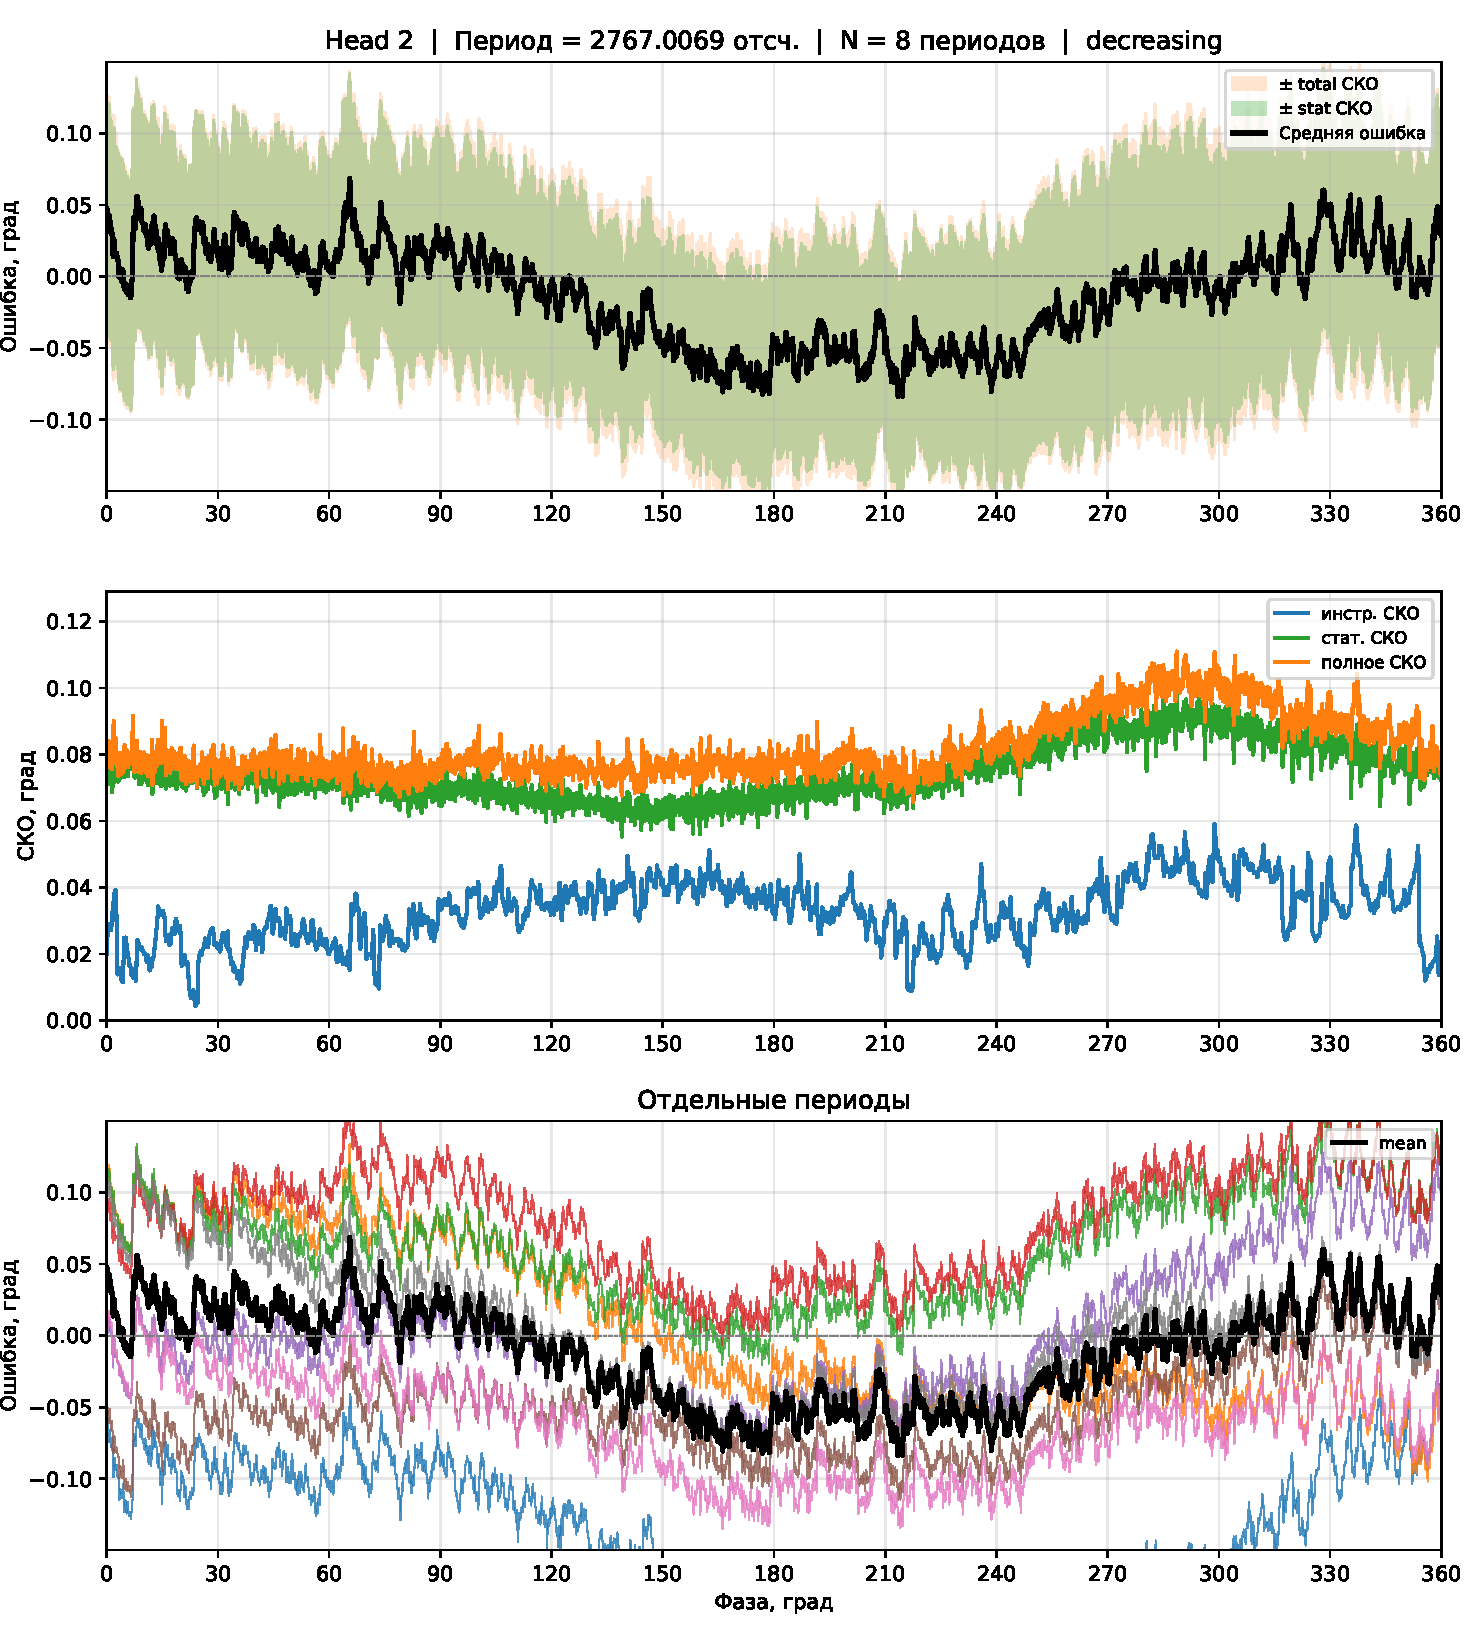
\includegraphics[width=\linewidth]{images/final_reverse10_5000_head2.pdf}
\caption{При скорости 5000 микрошагов в сек. (один оборот за $\sim62$ сек.) со второй головки при вращении противоположно считыванию}
\label{fig:profile5000}
\end{figure}

\begin{figure}[H]
\centering
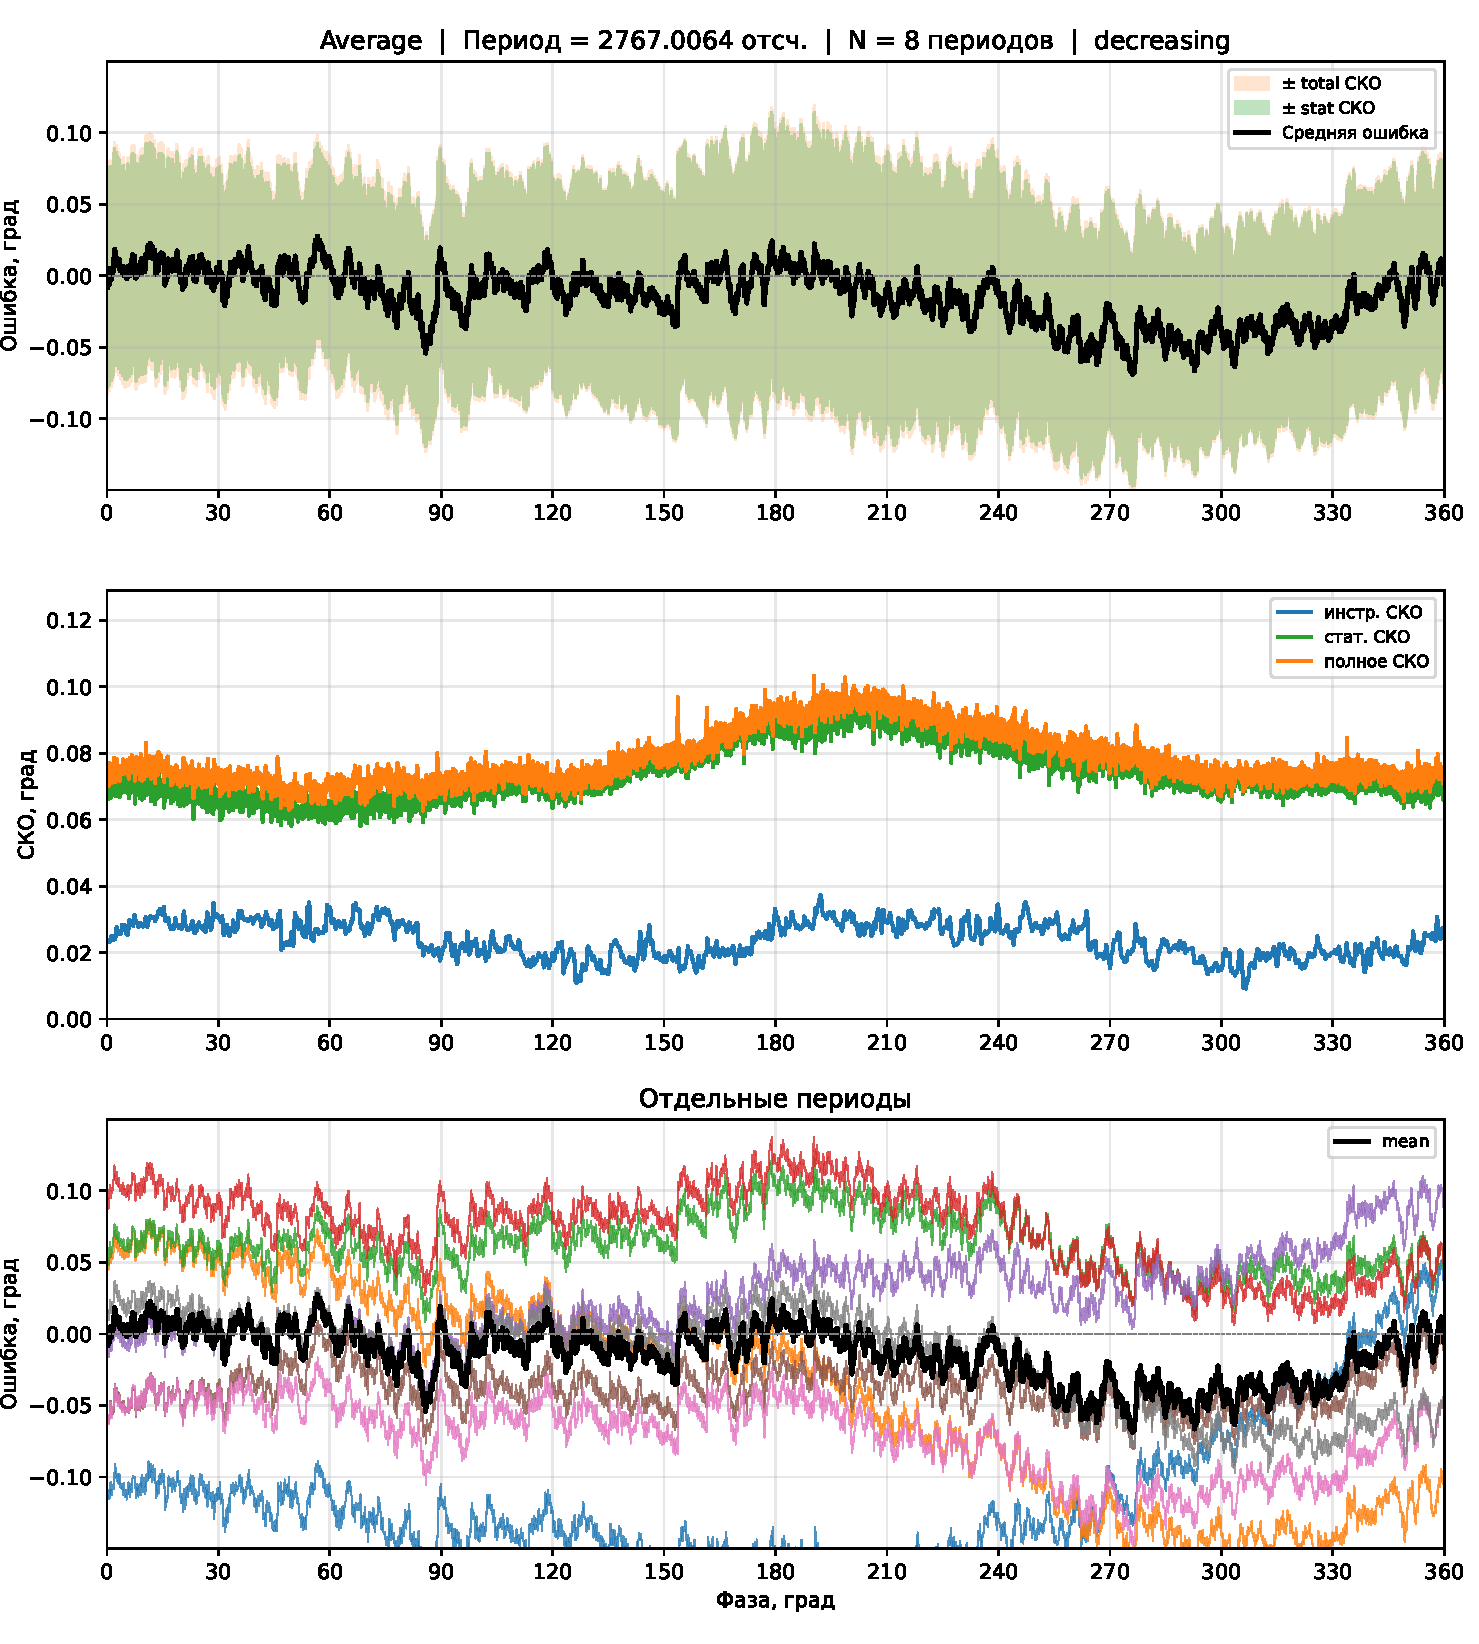
\includegraphics[width=\linewidth]{images/final_reverse10_5000_avg.pdf}
\caption{При скорости 5000 микрошагов в сек. (один оборот за $\sim62$ сек.) круговое среднее показаний двух головок при вращении противоположно считыванию} 
\label{fig:profilerev10000}
\end{figure}



